\newpage
\section{Билет 17. Основные уровни сетевых протоколов. Семиуровневая модель OSI. Сети пакетной коммутации. Маршрутизация сообщений.}

\textcolor{blue}{Клик сюда~\ref{part2}} к «Сети пакетной коммутации. Маршрутизация сообщений.»

\textbf{Протокол} -- это набор соглашений между разработчиками ПО и аппаратуры. Текст протокола отвечает на вопрос: «Что нужно сделать, чтобы программы и устройства могли взаимодействовать с другими программами/устройствами, поддерживающими протокол».

\textbf{OSI} (Open Systems Interconnection model) -- открытая сетевая модель.

Модель описывает, какие уровни должны быть в сети и какие функции выполняются на каждом из уровней. OSI модель разделяет все протоколы на 7 таких уровней:
\begin{enumerate}
\item Физический (Physical)
\item Канальный (Datalink)
\item Сетевой (Network)
\item Транспортный (Transport)
\item Сеансовый (Session)
\item Представительный (Presentation)
\item Прикладной (Application)
\end{enumerate}

Все они отвечают за определенную ступень процесса отправки сетевого сообщения, а также содержат в себе определенную информацию. Шаги выполняются, обособленно друг от друга. Модель OSI \textbf{не включает} описание протоколов; они определяются в отдельных стандартах.
\newline
\begin{figure}[H] \centering
	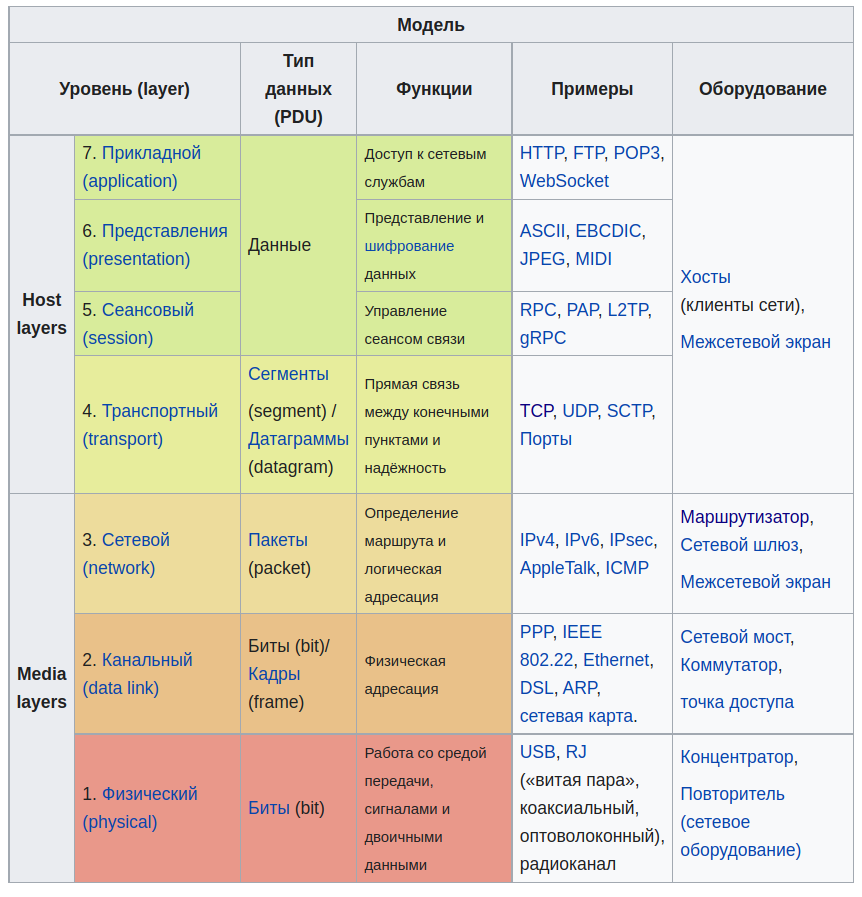
\includegraphics[scale = 0.6]{17/OSI.png}
	\caption{Уровни модели OSI}
\end{figure}

\textbf{Media layers} (уровни 1-3) управляют физической доставкой данных по сети.
\textbf{Host layers} (уровни 4-7) способствуют обеспечению точной доставки данных между компьютерами в сети.

\textbf{PDU} (Protocol data unit) -- это информация, доставляемая между одноуровневыми объектами сетей.

\textbf{Физический уровень} отвечает за обмен физическими сигналами между физическими устройствами. Основная его цель представить нуль и единицу в качестве сигналов, передаваемые по среде передачи данных. Никакой гарантии корректности передачи нет.

\textbf{Канальный уровень} предназначен для обеспечения взаимодействия сетей на физическом уровне и контроля ошибок, которые могут возникнуть. Канальный уровень получает (от физического уровня) биты, находит начало и конец сообщения и упаковывает биты в кадры (фреймы). проверяет их на целостность и, если нужно, исправляет ошибки (либо формирует повторный запрос повреждённого кадра) и отправляет на сетевой уровень. Задача здесь — сформировать кадры с адресом отправителя и получателя, после чего отправить их по сети.

У канального уровня есть два подуровня -- это MAC и LLC. MAC (Media Access Control, контроль доступа к среде) отвечает за присвоение физических MAC-адресов, а LLC (Logical Link Control, контроль логической связи) занимается проверкой и исправлением данных, управляет их передачей.

\textbf{Сетевой уровень} предназначен для определения пути передачи данных. Получает MAC-адрес от коммутаторов с предыдущего уровня и занимаются построением маршрута от одного устройства к другому с учетом всех потенциальных неполадок в сети. Преобразует физический адрес (MAC) в логический (IP).

\textbf{Транспортный уровень} предназначен для обеспечения надёжной передачи данных от отправителя к получателю (т.е. без потерь).

При передаче по протоколу TCP, данные делятся на сегменты. Сегмент -- это часть пакета. Когда приходит пакет данных, который превышает пропускную способность сети, пакет делится на сегменты допустимого размера. Сегментация пакетов также требуется в ненадежных сетях, когда существует большая вероятность того, что большой пакет будет потерян или отправлен не тому адресату.

При передаче данных по протоколу UDP, пакеты данных делятся уже на датаграммы. Датаграмма (datagram) -- это тоже часть пакета, но ее нельзя путать с сегментом. Главное отличие датаграмм в автономности. Каждая датаграмма содержит все необходимые заголовки, чтобы дойти до конечного адресата, поэтому они не зависят от сети, могут доставляться разными маршрутами и в разном порядке.

Датаграмма и сегмент -- это два PDU транспортного уровня модели OSI. При потере датаграмм или сегментов получаются «битые» куски данных, которые не получится корректно обработать.

\textbf{Сеансовый уровень} устанавливает и поддерживает продолжительные соединения, сеансы связи.
Уровень управляет созданием/завершением сеанса, обменом информацией, синхронизацией задач, определением права на передачу данных и поддержанием сеанса в периоды неактивности приложений.
Примером работы пятого уровня может служить видеозвонок по сети. Во время видеосвязи необходимо, чтобы два потока данных (аудио и видео) шли синхронно.

\textbf{Представительный уровень} занимается тем, что представляет данные (которые все еще являются PDU) в понятном человеку и машине виде. Например, когда одно устройство умеет отображать текст только в кодировке ASCII, а другое только в UTF-8, перевод текста из одной кодировки в другую происходит на шестом уровне.
Шестой уровень также занимается представлением картинок (в JPEG, GIF и т.д.), а также видео-аудио (в MPEG, QuickTime). Помимо перечисленного, шестой уровень занимается шифрованием данных, когда при передаче их необходимо защитить.

\textbf{Прикладной уровень} -- это ближайший уровень к пользователю. На нем реализуются протоколы на уровне приложений, такие как HTTP.  Его задача, визуализировать или записать данные, взаимодействовать с пользователем.

\textbf{Инкапсуляция} -- весь процесс преобразования данных (с верхнего уровня) в сигналы (на нижний уровень), обратный ему процесс называется \textbf{декапсуляцией}.

Исторически вышло, что на практике модель взаимодействия открытых систем не применяется. Раньше существовали её буквальные реализации, содержащие ровно 7 слоев. Однако со временем их вытеснил менее предписывающий набор протоколов TCP/IP, на котором построен современный Интернет. Тем не менее, модель OSI до сих пор используется в качестве эталона для обучения и документации.


\subsection*{Сети пакетной коммутации. Маршрутизация сообщений.}\label{b17:part2}

\textbf{Пакетная коммутации} -- процесс передачи пакетов с использованием транзитных узлов.

\textbf{Маршрутизация} -- процесс определения маршрута данных в сетях связи.

Хотим передать большой файл от A к B. Наше сообщение делится на пакеты, в соответствии с используемым протоколом.
А -> роутер -> маршрутизатор.
У одного маршрутизатора есть несколько физических входящих и исходящих каналов. Соответственно на один маршрутизатор могут приходить пакеты с разных узлов. Внутри маршрутизатора своя очередь приема пакетов и соответственно очередь передачи.
Задача маршрутизатора глядя на логические адреса (куда нужно доставить сообщение), выбрать оптимальный маршрут.

Очередь отправки может переполниться. (Лектор говорит, что очередь приёма не переполняется, так как время обработки пакета в маршрутизаторе согласовано с пропускной способностью.) Может случиться, что пакеты пришли с двух узлов, а отправить их маршрутизатор решил дальше по одному каналу -- в этот момент может произойти переполнение.
Маршрутизатору не хватает ресурсов запомнить все пакеты, которые нужно отправить, а пропускной способности соединения не хватает, чтобы отправить эти пакеты. В такой ситуации маршрутизатор может потерять пакет.

Когда передаем сообщение от А к В, это сообщение проходит через какое-то количество промежуточных устройств. Чем больше устройств, тем больше шанс потерять сообщение, тем больше задержка.

Внутри маршрутизатора строятся таблицы маршрутизации -- они помогают определять оптимальный путь сообщения. Так же в случае недоступности узла, спустя время все пути перестраиваются (для ещё не отправленных сообщений).